% answers.tex —— 2013 年·重庆卷·文科 · 参考答案与详细解析片段
% 由 tools/generate_projects.py 依来源总账自 2013/2013_数学真题_重庆文_试题.md + 2013/2013_数学真题_重庆文_解析正文.md + 2013/2013_数学真题_重庆文_答案要点.md 生成，勿手改（改源 MD 后重跑）

\begin{answer}
\gksolhead{1}{}

\textbf{题目}：

已知全集 $U=\{1,2,3,4\}$，集合 $A=\{1,2\}$，$B=\{2,3\}$，则 $\complement_U(A\cup B)=$\mbox{（　　）}
（A）$\{1,3,4\}$；（B）$\{3,4\}$；（C）$\{3\}$；（D）$\{4\}$。

\Needspace{4\baselineskip}
\textbf{解析}
\Needspace{5\baselineskip}
全集 $U=\{1,2,3,4\}$，而
\nopagebreak[4]
\[A\cup B=\{1,2\}\cup\{2,3\}=\{1,2,3\},\]
\Needspace{5\baselineskip}
故
\nopagebreak[4]
\[\complement_U(A\cup B)=\{4\}.\]
选 D。

\gkanswer{答案：D。}

\end{answer}
\begin{answer}
\gksolhead{2}{}

\textbf{题目}：

命题“对任意 $x\in\mathbf R$，都有 $x^2\geqslant0$”的否定为\mbox{（　　）}
（A）存在 $x_0\in\mathbf R$，使得 $x_0^2<0$；（B）不存在 $x\in\mathbf R$，使得 $x^2<0$；（C）存在 $x_0\in\mathbf R$，使得 $x_0^2\geqslant0$；（D）对任意 $x\in\mathbf R$，都有 $x^2<0$。

\Needspace{4\baselineskip}
\textbf{解析}
\Needspace{5\baselineskip}
命题“对任意 $x\in\mathbf R$，都有 $x^2\geqslant0$”是全称命题，其否定是特称命题：把全称量词“任意”改为存在量词“存在”，并把结论 $x^2\geqslant0$ 否定为 $x^2<0$，即
\nopagebreak[4]
\[\text{\text{存在} }x_0\in\mathbf R,\ \text{\text{使得} }x_0^2<0.\]
选 A。

\gkanswer{答案：A。}

\end{answer}
\begin{answer}
\gksolhead{3}{}

\textbf{题目}：

函数 $y=\dfrac1{\log_2(x-2)}$ 的定义域是\mbox{（　　）}
（A）$(-\infty,2)$；（B）$(2,+\infty)$；（C）$(2,3)\cup(3,+\infty)$；（D）$(2,4)\cup(4,+\infty)$。

\Needspace{4\baselineskip}
\textbf{解析}
\Needspace{5\baselineskip}
函数有意义须同时满足两个条件：
\nopagebreak[4]
\[\begin{cases}x-2>0,\\ \log_2(x-2)\neq0,\end{cases}\iff\begin{cases}x>2,\\ x-2\neq1,\end{cases}\iff x>2\ \text{\text{且}}\ x\neq3.\]
\Needspace{5\baselineskip}
故定义域为
\nopagebreak[4]
\[(2,3)\cup(3,+\infty).\]
选 C。

\gkanswer{答案：C。}

\end{answer}
\begin{answer}
\gksolhead{4}{}

\textbf{题目}：

设 $P$ 是圆 $(x-3)^2+(y+1)^2=4$ 上的动点，$Q$ 是直线 $x=-3$ 上的动点，则 $|PQ|$ 的最小值为\mbox{（　　）}
（A）$6$；（B）$4$；（C）$3$；（D）$2$。

\Needspace{4\baselineskip}
\textbf{解析}
\Needspace{5\baselineskip}
圆 $(x-3)^2+(y+1)^2=4$ 的圆心为 $C(3,-1)$，半径 $r=2$。点 $C$ 到直线 $x=-3$ 的距离为
\nopagebreak[4]
\[d=3-(-3)=6.\]
\Needspace{5\baselineskip}
对直线上任意一点 $Q$，由三角不等式 $|PQ|\geqslant|CQ|-|CP|\geqslant d-r$，且当 $P$ 取 $C$ 到直线的垂线段与圆的靠近直线的交点、$Q$ 取垂足时等号成立，故
\nopagebreak[4]
\[|PQ|_{\min}=d-r=6-2=4.\]
选 B。

\gkanswer{答案：B。}

\end{answer}
\begin{answer}
\gksolhead{5}{}

\textbf{题目}：

执行如图所示的程序框图，则输出的 $k$ 的值是\mbox{（　　）}
\nopagebreak[4]
\begin{center}% 2013 重庆卷文科第 5 题：输出 k 的值的程序框图。
\begin{tikzpicture}[font=\footnotesize, >=Stealth, line width=0.45pt,
  node distance=4.8mm,
  term/.style={draw, rounded corners=5pt, minimum height=1.8em, inner xsep=8pt},
  io/.style={draw, trapezium, trapezium left angle=72, trapezium right angle=108,
             minimum height=1.8em, inner xsep=7pt},
  box/.style={draw, minimum height=1.8em, inner xsep=6pt},
  dec/.style={draw, diamond, aspect=2.6, inner sep=1pt}]
  \node[term] (start) {开始};
  \node[box, below=5mm of start] (init) {$k=1$，$s=1$};
  \node[box, below=8mm of init] (acc) {$s=s+(k-1)^2$};
  \node[dec, below=6mm of acc] (test) {$s>15$?};
  \node[box, right=11mm of test] (inc) {$k=k+1$};
  \node[io, below=10mm of test] (output) {输出 $k$};
  \node[term, below=5mm of output] (end) {结束};
  \draw[->] (start) -- (init);
  \draw[->] (init) -- (acc);
  \draw[->] (acc) -- (test);
  \draw[->] (test) -- node[right] {是} (output);
  \draw[->] (test) -- node[above] {否} (inc);
  \draw[->] (output) -- (end);
  % 否分支回到累加框上方
  \coordinate (loop) at ($(acc.north)+(0.55,0.40)$);
  \coordinate (loopt) at ($(acc.north)+(0.55,0)$);
  \draw[->] (inc.north) -- (inc.north |- loop) -- (loop) -- (loopt);
\end{tikzpicture}
\end{center}
\nopagebreak[4]
（A）$3$；（B）$4$；（C）$5$；（D）$6$。

\Needspace{4\baselineskip}
\textbf{解析}
按框图顺序执行，注意判断框为“$s>15$?”，“是”时输出 $k$，“否”时 $k$ 增加 $1$ 后返回累加框：
\begin{center}
\begin{tabular}{lll}
\toprule
进入累加时的 $k$ & 累加后 $s=s+(k-1)^2$ & 判断 $s>15$ \\
\midrule
$1$ & $1+0=1$ & 否，$k$ 变为 $2$ \\
$2$ & $1+1=2$ & 否，$k$ 变为 $3$ \\
$3$ & $2+4=6$ & 否，$k$ 变为 $4$ \\
$4$ & $6+9=15$ & 否（$15>15$ 不成立），$k$ 变为 $5$ \\
$5$ & $15+16=31$ & 是，输出 $k=5$ \\
\bottomrule
\end{tabular}
\end{center}

故输出的 $k$ 的值是 $5$。选 C。

\gkanswer{答案：C。}

\end{answer}
\begin{answer}
\gksolhead{6}{}

\textbf{题目}：

如图是某公司 $10$ 个销售店某月销售某产品数量（单位：台）的茎叶图，则数据落在区间 $[22,30)$ 内的频率为\mbox{（　　）}
\nopagebreak[4]
\begin{center}% 2013 重庆卷文科第 6 题：10 个销售店某月销售某产品数量的茎叶图。
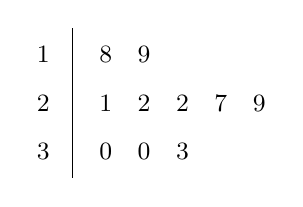
\begin{tikzpicture}[font=\small, line width=0.45pt]
  % 茎（十位）
  \node[anchor=east] at (0,0.62) {1};
  \node[anchor=east] at (0,0) {2};
  \node[anchor=east] at (0,-0.62) {3};
  % 分隔竖线
  \draw (0.16,0.95) -- (0.16,-0.95);
  % 叶（个位）
  \node[anchor=west] at (0.38,0.62) {8\quad 9};
  \node[anchor=west] at (0.38,0) {1\quad 2\quad 2\quad 7\quad 9};
  \node[anchor=west] at (0.38,-0.62) {0\quad 0\quad 3};
\end{tikzpicture}
\end{center}
\nopagebreak[4]
（A）$0.2$；（B）$0.4$；（C）$0.5$；（D）$0.6$。

\Needspace{4\baselineskip}
\textbf{解析}
\Needspace{5\baselineskip}
茎叶图共 $10$ 个数据，按十位（茎）与个位（叶）读出：
\nopagebreak[4]
\[18,\ 19;\qquad 21,\ 22,\ 22,\ 27,\ 29;\qquad 30,\ 30,\ 33.\]
\Needspace{5\baselineskip}
其中落在 $[22,30)$ 内的数据为 $22,\ 22,\ 27,\ 29$，共 $4$ 个，故频率为
\nopagebreak[4]
\[\frac4{10}=0.4.\]
选 B。

\gkanswer{答案：B。}

\end{answer}
\begin{answer}
\gksolhead{7}{}

\textbf{题目}：

关于 $x$ 的不等式 $x^2-2ax-8a^2<0$（$a>0$）的解集为 $(x_1,x_2)$，且 $x_2-x_1=15$，则 $a=$\mbox{（　　）}
（A）$\dfrac52$；（B）$\dfrac72$；（C）$\dfrac{15}4$；（D）$\dfrac{15}2$。

\Needspace{4\baselineskip}
\textbf{解析}
\Needspace{5\baselineskip}
因式分解：
\nopagebreak[4]
\[x^2-2ax-8a^2=(x-4a)(x+2a).\]
\Needspace{5\baselineskip}
由 $a>0$ 得 $-2a<4a$，故不等式的解集为
\nopagebreak[4]
\[(-2a,4a),\qquad x_1=-2a,\quad x_2=4a.\]
\Needspace{5\baselineskip}
于是
\nopagebreak[4]
\[x_2-x_1=4a-(-2a)=6a=15\implies a=\frac52.\]
选 A。

\gkanswer{答案：A。}

\end{answer}
\begin{answer}
\gksolhead{8}{}

\textbf{题目}：

某几何体的三视图如图所示，则该几何体的表面积为\mbox{（　　）}
\nopagebreak[4]
\begin{center}% 2013 重庆卷文科第 8 题：几何体的三视图。
% 正（主）视图为 10×4 的矩形；侧（左）视图为下底 8、上底 2、高 4 的等腰梯形；
% 俯视图为 10×8 的矩形，被两条与长边平行的线分成 3、2、3 三部分。
\begin{tikzpicture}[font=\small, >=Stealth, line width=0.45pt, x=0.26cm, y=0.26cm]
  % ---- 正（主）视图：10 宽、4 高 ----
  \draw (0,0) rectangle (10,4);
  % 尺寸 4
  \draw[<->] (-2,0) -- (-2,4);
  \draw (-2.8,0) -- (-1.2,0);
  \draw (-2.8,4) -- (-1.2,4);
  \node[left] at (-2.8,2) {4};
  % 尺寸 10
  \draw[<->] (0,-2) -- (10,-2);
  \draw (0,-2.8) -- (0,-1.2);
  \draw (10,-2.8) -- (10,-1.2);
  \node[below] at (5,-2.2) {10};
  \node[below] at (5,-3.6) {正（主）视图};

  % ---- 侧（左）视图：下底 8、上底 2、高 4 的等腰梯形 ----
  \begin{scope}[shift={(13.8,0)}]
    \draw (0,0) -- (8,0) -- (5,4) -- (3,4) -- cycle;
    \draw[<->] (0,-2) -- (8,-2);
    \draw (0,-2.8) -- (0,-1.2);
    \draw (8,-2.8) -- (8,-1.2);
    \node[below] at (4,-2.2) {8};
    \node[below] at (4,-3.6) {侧（左）视图};
  \end{scope}

  % ---- 俯视图：10×8 的矩形，分成 3、2、3 ----
  \begin{scope}[shift={(0,-14)}]
    \draw (0,0) rectangle (10,8);
    \draw (0,5.7) -- (10,5.7);
    \draw (0,3.3) -- (10,3.3);
    % 左侧尺寸 3、2、3
    \draw[<->] (-2,5.7) -- (-2,8);
    \draw[<->] (-2,3.3) -- (-2,5.7);
    \draw[<->] (-2,0) -- (-2,3.3);
    \draw (-2.8,0) -- (-1.2,0);
    \draw (-2.8,3.3) -- (-1.2,3.3);
    \draw (-2.8,5.7) -- (-1.2,5.7);
    \draw (-2.8,8) -- (-1.2,8);
    \node[left] at (-2.8,6.85) {3};
    \node[left] at (-2.8,4.5) {2};
    \node[left] at (-2.8,1.65) {3};
    \node[below] at (5,-1.4) {俯视图};
  \end{scope}
\end{tikzpicture}
\end{center}
\nopagebreak[4]
（A）$180$；（B）$200$；（C）$220$；（D）$240$。

\Needspace{4\baselineskip}
\textbf{解析}
由三视图还原几何体：正（主）视图是 $10\times4$ 的矩形，说明几何体高 $4$、沿正前方投影长 $10$；侧（左）视图是下底 $8$、上底 $2$、高 $4$ 的等腰梯形；俯视图是 $10\times8$ 的矩形，被两条平行于长边的线分成 $3$、$2$、$3$ 三部分，正与梯形上底 $2$、两腰水平投影各 $3$ 对应。
因此该几何体是一个横放的直棱柱：底面为上述等腰梯形，棱柱的高（长度）为 $10$。

\Needspace{5\baselineskip}
梯形的两腰长为
\nopagebreak[4]
\[\sqrt{3^2+4^2}=5.\]
\Needspace{5\baselineskip}
表面积由两个梯形底面、下底面、上底面和两个侧面组成：
\nopagebreak[4]
\[S=2\times\frac{8+2}2\times4+8\times10+2\times10+2\times(5\times10).\]
\Needspace{5\baselineskip}
逐项计算：
\nopagebreak[4]
\[S=2\times20+80+20+2\times50=40+80+20+100=240.\]
选 D。

\gkanswer{答案：D。}

\end{answer}
\begin{answer}
\gksolhead{9}{}

\textbf{题目}：

已知函数 $f(x)=ax^3+b\sin x+4$（$a,b\in\mathbf R$），$f(\lg(\log_2 10))=5$，则 $f(\lg(\lg 2))=$\mbox{（　　）}
（A）$-5$；（B）$-1$；（C）$3$；（D）$4$。

\Needspace{4\baselineskip}
\textbf{解析}
\Needspace{5\baselineskip}
令 $g(x)=ax^3+b\sin x$，则 $g(-x)=-g(x)$，即 $g$ 为奇函数，且
\nopagebreak[4]
\[f(x)=g(x)+4,\qquad f(x)+f(-x)=g(x)+g(-x)+8=8.\]
\Needspace{5\baselineskip}
又
\nopagebreak[4]
\[\log_2 10=\frac1{\log_{10}2}=\frac1{\lg2},\]
\Needspace{5\baselineskip}
故
\nopagebreak[4]
\[\lg(\log_2 10)=\lg\frac1{\lg2}=-\lg(\lg2).\]
\Needspace{5\baselineskip}
记 $t=\lg(\lg2)$，则 $f(-t)=f(\lg(\log_2 10))=5$，于是
\nopagebreak[4]
\[f(t)=8-f(-t)=8-5=3,\]
即 $f(\lg(\lg2))=3$。选 C。

\gkanswer{答案：C。}

\end{answer}
\begin{answer}
\gksolhead{10}{}

\textbf{题目}：

设双曲线 $C$ 的中心为点 $O$，若有且只有一对相交于点 $O$、所成的角为 $60^\circ$ 的直线 $A_1B_1$ 和 $A_2B_2$，使 $|A_1B_1|=|A_2B_2|$，其中 $A_1$，$B_1$ 和 $A_2$，$B_2$ 分别是这对直线与双曲线 $C$ 的交点，则该双曲线的离心率的取值范围是\mbox{（　　）}
（A）$\left(\dfrac{2\sqrt3}3,2\right]$；（B）$\left[\dfrac{2\sqrt3}3,2\right)$；（C）$\left(\dfrac{2\sqrt3}3,+\infty\right)$；（D）$\left[\dfrac{2\sqrt3}3,+\infty\right)$。

\Needspace{4\baselineskip}
\textbf{解析}
\Needspace{5\baselineskip}
设双曲线 $C$ 的方程为 $\dfrac{x^2}{a^2}-\dfrac{y^2}{b^2}=1$（$a,b>0$），离心率
\nopagebreak[4]
\[e=\sqrt{1+\frac{b^2}{a^2}}.\]

\Needspace{5\baselineskip}
先看一条过 $O$ 的直线与 $C$ 的交弦。竖直线 $x=0$ 与 $C$ 无交点；设直线为 $y=kx$，代入得
\nopagebreak[4]
\[x^2\left(\frac1{a^2}-\frac{k^2}{b^2}\right)=1.\]
\Needspace{5\baselineskip}
它有两个交点当且仅当
\nopagebreak[4]
\[\frac1{a^2}-\frac{k^2}{b^2}>0\iff |k|<\frac ba.\]
\Needspace{5\baselineskip}
此时两交点关于 $O$ 对称，弦长为
\nopagebreak[4]
\[L(k)=2\sqrt{1+k^2}\cdot\frac1{\sqrt{\frac1{a^2}-\frac{k^2}{b^2}}}.\]
\Needspace{5\baselineskip}
$L$ 只与 $|k|$ 有关，且
\nopagebreak[4]
\[L^2=\frac{4(1+k^2)}{\frac1{a^2}-\frac{k^2}{b^2}}\]
的分子随 $k^2$ 增大而增大、分母随 $k^2$ 增大而减小，故 $L$ 在 $[0,\frac ba)$ 上关于 $|k|$ 严格递增。

因此 $|A_1B_1|=|A_2B_2|$ 当且仅当 $|k_1|=|k_2|$；两直线不同，故 $k_2=-k_1$，即这一对直线关于 $x$ 轴对称。

\Needspace{5\baselineskip}
设 $|k|=\tan\theta$，$\theta\in\left(0,\dfrac\pi2\right)$。直线 $y=\pm kx$ 的倾斜角分别为 $\theta$ 与 $\pi-\theta$，两条直线所成的角为
\nopagebreak[4]
\[\min\{2\theta,\ \pi-2\theta\}.\]
\Needspace{5\baselineskip}
要求它为 $60^\circ$，则
\nopagebreak[4]
\[2\theta=60^\circ\ \text{\text{或}}\ \pi-2\theta=60^\circ,\]
\Needspace{5\baselineskip}
即 $\theta=30^\circ$ 或 $\theta=60^\circ$，从而
\nopagebreak[4]
\[|k|=\frac1{\sqrt3}\quad\text{\text{或}}\quad |k|=\sqrt3.\]

所以满足“弦长相等且夹角为 $60^\circ$”的直线对至多有两对，分别对应 $|k|=\dfrac1{\sqrt3}$ 与 $|k|=\sqrt3$。其中某一对真实存在，当且仅当相应斜率满足 $|k|<\dfrac ba$。

\Needspace{5\baselineskip}
题设要求“有且只有一对”，即 $\dfrac1{\sqrt3}$ 与 $\sqrt3$ 中恰有一个小于 $\dfrac ba$：
\nopagebreak[4]
\[\frac1{\sqrt3}<\frac ba\leqslant\sqrt3.\]
（若 $\dfrac ba\leqslant\dfrac1{\sqrt3}$ 则一对也没有；若 $\dfrac ba>\sqrt3$ 则两对都存在。）

\Needspace{5\baselineskip}
于是
\nopagebreak[4]
\[\frac13<\frac{b^2}{a^2}\leqslant3,\qquad e^2=1+\frac{b^2}{a^2}\in\left(\frac43,4\right],\]
\Needspace{5\baselineskip}
故
\nopagebreak[4]
\[e\in\left(\frac{2\sqrt3}3,2\right].\]
选 A。

\gkanswer{答案：A。}

\end{answer}
\begin{answer}
\gksolhead{11}{}

\textbf{题目}：

设复数 $z=1+2\mathrm i$（$\mathrm i$ 是虚数单位），则 $|z|=$\gkblank{}。

\Needspace{4\baselineskip}
\textbf{解析}
\Needspace{5\baselineskip}
由复数模的定义，
\nopagebreak[4]
\[|z|=|1+2\mathrm i|=\sqrt{1^2+2^2}=\sqrt5.\]
填 $\sqrt5$。

\gkanswer{答案：$\sqrt5$。}

\end{answer}
\begin{answer}
\gksolhead{12}{}

\textbf{题目}：

若 $2$，$a$，$b$，$c$，$9$ 成等差数列，则 $c-a=$\gkblank{}。

\Needspace{4\baselineskip}
\textbf{解析}
\Needspace{5\baselineskip}
$2,a,b,c,9$ 成等差数列，设公差为 $d$，则
\nopagebreak[4]
\[9=2+4d\implies d=\frac74.\]
\Needspace{5\baselineskip}
于是
\nopagebreak[4]
\[a=2+d,\qquad c=2+3d,\]
\nopagebreak[4]
\[c-a=2d=\frac72.\]
填 $\dfrac72$。

\gkanswer{答案：$\dfrac72$。}

\end{answer}
\begin{answer}
\gksolhead{13}{}

\textbf{题目}：

若甲、乙、丙三人随机地站成一排，则甲、乙两人相邻而站的概率为\gkblank{}。

\Needspace{4\baselineskip}
\textbf{解析}
\Needspace{5\baselineskip}
三人随机站成一排共有
\nopagebreak[4]
\[3!=6\]
\Needspace{5\baselineskip}
种等可能的站法。甲、乙相邻时，把甲、乙看成一个整体，与丙共两个元素排列有 $2!$ 种，甲、乙内部又有 $2!$ 种顺序，故有利站法
\nopagebreak[4]
\[2!\times2!=4\]
\Needspace{5\baselineskip}
种。所求概率为
\nopagebreak[4]
\[P=\frac46=\frac23.\]
填 $\dfrac23$。

\gkanswer{答案：$\dfrac23$。}

\end{answer}
\begin{answer}
\gksolhead{14}{}

\textbf{题目}：

在 $\overrightarrow{OA}$ 为边、$\overrightarrow{OB}$ 为对角线的矩形中，已知 $\overrightarrow{OA}=(-3,1)$，$\overrightarrow{OB}=(-2,k)$，则实数 $k=$\gkblank{}。

\Needspace{4\baselineskip}
\textbf{解析}
\Needspace{5\baselineskip}
以 $\overrightarrow{OA}$ 为一边、$\overrightarrow{OB}$ 为对角线的矩形中，另一邻边为
\nopagebreak[4]
\[\overrightarrow{AB}=\overrightarrow{OB}-\overrightarrow{OA}=(-2,k)-(-3,1)=(1,k-1).\]
\Needspace{5\baselineskip}
矩形中 $\overrightarrow{AB}\perp\overrightarrow{OA}$，故
\nopagebreak[4]
\[\overrightarrow{AB}\cdot\overrightarrow{OA}=1\times(-3)+(k-1)\times1=0,\]
\Needspace{5\baselineskip}
即
\nopagebreak[4]
\[-3+k-1=0\implies k=4.\]
填 $4$。

\gkanswer{答案：$4$。}

\end{answer}
\begin{answer}
\gksolhead{15}{}

\textbf{题目}：

设 $0\leqslant\alpha\leqslant\pi$，不等式 $8x^2-(8\sin\alpha)x+\cos2\alpha\geqslant0$ 对 $x\in\mathbf R$ 恒成立，则 $\alpha$ 的取值范围为\gkblank{}。

\Needspace{4\baselineskip}
\textbf{解析}
\Needspace{5\baselineskip}
设 $f(x)=8x^2-(8\sin\alpha)x+\cos2\alpha$。因二次项系数 $8>0$，$f(x)\geqslant0$ 对一切 $x\in\mathbf R$ 恒成立当且仅当判别式
\nopagebreak[4]
\[\Delta=(8\sin\alpha)^2-4\times8\cos2\alpha\leqslant0.\]
\Needspace{5\baselineskip}
即
\nopagebreak[4]
\[64\sin^2\alpha-32\cos2\alpha\leqslant0.\]
\Needspace{5\baselineskip}
两边除以 $32$，并用 $\cos2\alpha=1-2\sin^2\alpha$：
\nopagebreak[4]
\[2\sin^2\alpha-(1-2\sin^2\alpha)\leqslant0\iff4\sin^2\alpha\leqslant1,\]
\Needspace{5\baselineskip}
故
\nopagebreak[4]
\[\sin^2\alpha\leqslant\frac14\iff-\frac12\leqslant\sin\alpha\leqslant\frac12.\]
\Needspace{5\baselineskip}
由 $0\leqslant\alpha\leqslant\pi$ 得
\nopagebreak[4]
\[\alpha\in\left[0,\frac\pi6\right]\cup\left[\frac{5\pi}6,\pi\right].\]
填 $\left[0,\dfrac\pi6\right]\cup\left[\dfrac{5\pi}6,\pi\right]$。

\gkanswer{答案：$\left[0,\dfrac\pi6\right]\cup\left[\dfrac{5\pi}6,\pi\right]$。}

\end{answer}
\begin{answer}
\gksolhead{16}{}

\textbf{题目}：

设数列 $\{a_n\}$ 满足：$a_1=1$，$a_{n+1}=3a_n$，$n\in\mathbf N_+$。
（1） 求 $\{a_n\}$ 的通项公式及前 $n$ 项和 $S_n$；
（2） 已知 $\{b_n\}$ 是等差数列，$T_n$ 为其前 $n$ 项和，且 $b_1=a_2$，$b_3=a_1+a_2+a_3$，求 $T_{20}$。

\Needspace{4\baselineskip}
\textbf{解析}
\Needspace{5\baselineskip}
\textbf{（1）} 由 $a_{n+1}=3a_n$ 且 $a_1=1\neq0$ 知 $\{a_n\}$ 是首项为 $1$、公比为 $3$ 的等比数列，故
\nopagebreak[4]
\[a_n=1\times3^{n-1}=3^{n-1}.\]
\Needspace{5\baselineskip}
前 $n$ 项和
\nopagebreak[4]
\[S_n=\frac{1\cdot(3^n-1)}{3-1}=\frac{3^n-1}2.\]
\Needspace{5\baselineskip}
\textbf{（2）} 由（1）得 $a_1=1$，$a_2=3$，$a_3=9$，于是
\nopagebreak[4]
\[b_1=a_2=3,\qquad b_3=a_1+a_2+a_3=1+3+9=13.\]
\Needspace{5\baselineskip}
设 $\{b_n\}$ 的公差为 $d$，则
\nopagebreak[4]
\[b_3=b_1+2d\implies13=3+2d\implies d=5.\]
\Needspace{5\baselineskip}
故
\nopagebreak[4]
\[T_{20}=20b_1+\frac{20\times19}2d=20\times3+190\times5=60+950=1010.\]

\gkanswer{答案（1）：$a_n=3^{n-1}$，$S_n=\dfrac{3^n-1}2$。}

\gkanswer{答案（2）：$T_{20}=1010$。}

\end{answer}
\begin{answer}
\gksolhead{17}{}

\textbf{题目}：

从某居民区随机抽取 $10$ 个家庭，获得第 $i$ 个家庭的月收入 $x_i$（单位：千元）与月储蓄 $y_i$（单位：千元）的数据资料，算得 $\sum\limits_{i=1}^{10}x_i=80$，$\sum\limits_{i=1}^{10}y_i=20$，$\sum\limits_{i=1}^{10}x_iy_i=184$，$\sum\limits_{i=1}^{10}x_i^2=720$。
（1） 求家庭的月储蓄 $y$ 对月收入 $x$ 的线性回归方程 $\hat y=\hat bx+\hat a$；
（2） 判断变量 $x$ 与 $y$ 之间是正相关还是负相关；
（3） 若该居民区某家庭月收入为 $7$ 千元，预测该家庭的月储蓄。
附：线性回归方程 $\hat y=\hat bx+\hat a$ 中，$\hat b=\dfrac{\sum\limits_{i=1}^n x_iy_i-n\bar x\bar y}{\sum\limits_{i=1}^n x_i^2-n\bar x^2}$，$\hat a=\bar y-\hat b\bar x$，其中 $\bar x$，$\bar y$ 为样本平均值，线性回归方程也可写为 $\hat y=\hat bx+\hat a$。

\Needspace{4\baselineskip}
\textbf{解析}
\Needspace{5\baselineskip}
\textbf{（1）} 样本量 $n=10$，故
\nopagebreak[4]
\[\bar x=\frac{80}{10}=8,\qquad \bar y=\frac{20}{10}=2.\]
\Needspace{5\baselineskip}
由题给和式数据，
\nopagebreak[4]
\[\hat b=\frac{\sum\limits_{i=1}^{10}x_iy_i-10\bar x\bar y}{\sum\limits_{i=1}^{10}x_i^2-10\bar x^2}
=\frac{184-10\times8\times2}{720-10\times8^2}
=\frac{184-160}{720-640}=\frac{24}{80}=\frac3{10}.\]
\nopagebreak[4]
\[\hat a=\bar y-\hat b\bar x=2-\frac3{10}\times8=2-\frac{12}5=-\frac25.\]
\Needspace{5\baselineskip}
故线性回归方程为
\nopagebreak[4]
\[\hat y=0.3x-0.4.\]
\textbf{（2）} 因 $\hat b=0.3>0$，变量 $x$ 与 $y$ 正相关。
\Needspace{5\baselineskip}
\textbf{（3）} 当 $x=7$ 时，
\nopagebreak[4]
\[\hat y=0.3\times7-0.4=2.1-0.4=1.7,\]
即预测该家庭的月储蓄为 $1.7$ 千元。

\gkanswer{答案（1）：$\hat y=0.3x-0.4$。}

\gkanswer{答案（2）：正相关。}

\gkanswer{答案（3）：$1.7$ 千元。}

\end{answer}
\begin{answer}
\gksolhead{18}{}

\textbf{题目}：

在 $\triangle ABC$ 中，内角 $A$，$B$，$C$ 的对边分别为 $a$，$b$，$c$，且 $a^2=b^2+c^2+\sqrt3bc$。
（1） 求 $A$；
（2） 设 $a=\sqrt3$，$S$ 为 $\triangle ABC$ 的面积，求 $S+\sqrt3\cos B\cos C$ 的最大值，并指出此时 $B$ 的值。

\Needspace{4\baselineskip}
\textbf{解析}
\Needspace{5\baselineskip}
\textbf{（1）} 由余弦定理
\nopagebreak[4]
\[a^2=b^2+c^2-2bc\cos A.\]
\Needspace{5\baselineskip}
与题设 $a^2=b^2+c^2+\sqrt3bc$ 比较得
\nopagebreak[4]
\[-2bc\cos A=\sqrt3bc\implies\cos A=-\frac{\sqrt3}2.\]
\Needspace{5\baselineskip}
因 $A\in(0,\pi)$，故
\nopagebreak[4]
\[A=\frac{5\pi}6.\]
\Needspace{5\baselineskip}
\textbf{（2）} 由 $A=\dfrac{5\pi}6$ 得 $\sin A=\dfrac12$，故
\nopagebreak[4]
\[S=\frac12bc\sin A=\frac{bc}4.\]
\Needspace{5\baselineskip}
又 $B+C=\pi-A=\dfrac\pi6$，于是
\nopagebreak[4]
\[\cos B\cos C=\frac12\big[\cos(B+C)+\cos(B-C)\big]=\frac12\left[\frac{\sqrt3}2+\cos(B-C)\right].\]
\Needspace{5\baselineskip}
所以
\nopagebreak[4]
\[S+\sqrt3\cos B\cos C=\frac{bc}4+\frac34+\frac{\sqrt3}2\cos(B-C).\]
\Needspace{5\baselineskip}
由 $a=\sqrt3$ 及 $a^2=b^2+c^2+\sqrt3bc$ 得
\nopagebreak[4]
\[b^2+c^2+\sqrt3bc=3.\]
\Needspace{5\baselineskip}
而 $b^2+c^2\geqslant2bc$，故
\nopagebreak[4]
\[(2+\sqrt3)bc\leqslant3\implies bc\leqslant\frac3{2+\sqrt3}=3(2-\sqrt3)=6-3\sqrt3,\]
等号当且仅当 $b=c$ 时成立。
\Needspace{5\baselineskip}
又 $\cos(B-C)\leqslant1$，等号当且仅当 $B=C$ 时成立；而 $b=c$ 恰好给出 $B=C$，两处等号可同时取到。故
\nopagebreak[4]
\[S+\sqrt3\cos B\cos C\leqslant\frac{6-3\sqrt3}4+\frac34+\frac{\sqrt3}2=\frac{6-3\sqrt3+3+2\sqrt3}4=\frac{9-\sqrt3}4.\]
当 $b=c$、即 $B=C=\dfrac{\pi-A}2=\dfrac\pi{12}$ 时取到最大值 $\dfrac{9-\sqrt3}4$。

\gkanswer{答案（1）：$A=\dfrac{5\pi}6$。}

\gkanswer{答案（2）：最大值为 $\dfrac{9-\sqrt3}4$，此时 $B=C=\dfrac\pi{12}$。}

\end{answer}
\begin{answer}
\gksolhead{19}{}

\textbf{题目}：

如图，四棱锥 $P-ABCD$ 中，$PA\perp$ 底面 $ABCD$，$PA=2\sqrt3$，$BC=CD=2$，$\angle ACB=\angle ACD=\dfrac\pi3$。
\nopagebreak[4]
\begin{center}% 2013 重庆卷文科第 19 题：四棱锥 P-ABCD，PA 垂直于底面，
% F 在棱 PC 上且 PF=7FC。
\begin{tikzpicture}[font=\small, line width=0.45pt, scale=1]
  \coordinate (P) at (-0.15,3.40);
  \coordinate (A) at (0,0);
  \coordinate (B) at (1.60,-1.50);
  \coordinate (C) at (4.10,-0.70);
  \coordinate (D) at (3.20,1.40);
  \coordinate (F) at ($(P)!0.875!(C)$);
  % 可见棱
  \draw (P) -- (A);
  \draw (P) -- (B);
  \draw (P) -- (C);
  \draw (P) -- (D);
  \draw (A) -- (B);
  \draw (B) -- (C);
  \draw (C) -- (D);
  \draw (D) -- (A);
  % 不可见棱
  \draw[dashed] (A) -- (C);
  \draw[dashed] (B) -- (D);
  \draw[dashed] (B) -- (F);
  % 顶点标注
  \node[above left] at (P) {$P$};
  \node[below left] at (A) {$A$};
  \node[below] at (B) {$B$};
  \node[right] at (C) {$C$};
  \node[above right] at (D) {$D$};
  \node[left] at (F) {$F$};
\end{tikzpicture}
\end{center}
\nopagebreak[4]
（1） 求证：$BD\perp$ 平面 $PAC$；
（2） 若侧棱 $PC$ 上的点 $F$ 满足 $PF=7FC$，求三棱锥 $P-BDF$ 的体积。

\Needspace{4\baselineskip}
\textbf{解析}
\Needspace{5\baselineskip}
\textbf{（1）} 在 $\triangle BCD$ 中，$BC=CD=2$，故 $\triangle BCD$ 为等腰三角形。又
\nopagebreak[4]
\[\angle BCD=\angle ACB+\angle ACD=\frac\pi3+\frac\pi3=\frac{2\pi}3,\]
\Needspace{5\baselineskip}
且 $\angle ACB=\angle ACD$，即 $CA$ 是顶角 $\angle BCD$ 的平分线。由等腰三角形“三线合一”，
\nopagebreak[4]
\[CA\perp BD.\]
\Needspace{5\baselineskip}
因为 $PA\perp$ 平面 $ABCD$，$BD\subset$ 平面 $ABCD$，所以
\nopagebreak[4]
\[PA\perp BD.\]
\Needspace{5\baselineskip}
又 $PA\cap CA=A$，且 $PA$，$CA\subset$ 平面 $PAC$，由线面垂直的判定定理得
\nopagebreak[4]
\[BD\perp\text{\text{平面} }PAC.\]
\Needspace{5\baselineskip}
\textbf{（2）} 先求 $\triangle BCD$ 的面积：
\nopagebreak[4]
\[S_{\triangle BCD}=\frac12\cdot BC\cdot CD\cdot\sin\angle BCD=\frac12\times2\times2\times\sin\frac{2\pi}3=\frac12\times4\times\frac{\sqrt3}2=\sqrt3.\]
\Needspace{5\baselineskip}
三棱锥 $P-BCD$ 以 $BCD$ 为底、$PA$ 为高（因 $PA\perp$ 平面 $ABCD$），故
\nopagebreak[4]
\[V_{P-BCD}=\frac13S_{\triangle BCD}\cdot PA=\frac13\times\sqrt3\times2\sqrt3=2.\]
\Needspace{5\baselineskip}
由 $PF=7FC$ 得 $PF:FC=7:1$，故
\nopagebreak[4]
\[\frac{PF}{PC}=\frac78.\]
\Needspace{5\baselineskip}
三棱锥 $P-BDF$ 就是三棱锥 $B-PDF$。以 $B$ 为顶点、$\triangle PDF$ 为底：点 $F$ 在 $PC$ 上，$\triangle PDF$ 与 $\triangle PDC$ 都以 $D$ 为顶点、底边落在直线 $PC$ 上，故二者同高（点 $D$ 到直线 $PC$ 的距离），底边之比
\nopagebreak[4]
\[\frac{S_{\triangle PDF}}{S_{\triangle PDC}}=\frac{PF}{PC}=\frac78,\]
\Needspace{5\baselineskip}
且点 $B$ 到平面 $PCD$ 的距离不变，因此
\nopagebreak[4]
\[V_{P-BDF}=V_{B-PDF}=\frac78V_{B-PCD}=\frac78V_{P-BCD}=\frac78\times2=\frac74.\]
即三棱锥 $P-BDF$ 的体积为 $\dfrac74$。

\gkanswer{答案（1）：见解析版}

\gkanswer{答案（2）：$\dfrac74$。}

\end{answer}
\begin{answer}
\gksolhead{20}{}

\textbf{题目}：

某村庄拟修建一个无盖的圆柱形蓄水池（不计厚度）。设该蓄水池的底面半径为 $r$ 米，高为 $h$ 米，体积为 $V$ 立方米。假设建造成本仅与表面积有关，侧面的建造成本为 $100$ 元/平方米，底面的建造成本为 $160$ 元/平方米，该蓄水池的总建造成本为 $12000\pi$ 元（$\pi$ 为圆周率）。
（1） 将 $V$ 表示成 $r$ 的函数 $V(r)$，并求该函数的定义域；
（2） 讨论函数 $V(r)$ 的单调性，并确定 $r$ 和 $h$ 为何值时该蓄水池的体积最大。

\Needspace{4\baselineskip}
\textbf{解析}
\Needspace{5\baselineskip}
\textbf{（1）} 蓄水池无盖，侧面积为 $2\pi rh$，底面积为 $\pi r^2$，故总建造成本为
\nopagebreak[4]
\[100\times2\pi rh+160\times\pi r^2=12000\pi.\]
\Needspace{5\baselineskip}
两边除以 $40\pi$：
\nopagebreak[4]
\[5rh+4r^2=300\implies h=\frac{300-4r^2}{5r}.\]
\Needspace{5\baselineskip}
于是
\nopagebreak[4]
\[V(r)=\pi r^2h=\pi r^2\cdot\frac{300-4r^2}{5r}=\frac\pi5(300r-4r^3).\]
\Needspace{5\baselineskip}
由 $h>0$ 得 $300-4r^2>0$，即 $r<5\sqrt3$；又 $r>0$，故定义域为
\nopagebreak[4]
\[(0,5\sqrt3).\]
\Needspace{5\baselineskip}
\textbf{（2）} 求导：
\nopagebreak[4]
\[V'(r)=\frac\pi5(300-12r^2)=\frac{12\pi}5(25-r^2).\]
当 $0<r<5$ 时 $V'(r)>0$；当 $5<r<5\sqrt3$ 时 $V'(r)<0$。故 $V(r)$ 在 $(0,5)$ 上单调递增，在 $(5,5\sqrt3)$ 上单调递减，在 $r=5$ 处取得最大值。
\Needspace{5\baselineskip}
此时
\nopagebreak[4]
\[h=\frac{300-4\times25}{5\times5}=\frac{200}{25}=8,\]
\nopagebreak[4]
\[V(5)=\pi\times5^2\times8=200\pi.\]
即当 $r=5$ 米、$h=8$ 米时蓄水池的体积最大，最大体积为 $200\pi$ 立方米。

\gkanswer{答案（1）：$V(r)=\dfrac\pi5(300r-4r^3)$，定义域为 $(0,5\sqrt3)$。}

\gkanswer{答案（2）：$V(r)$ 在 $(0,5)$ 上单调递增，在 $(5,5\sqrt3)$ 上单调递减；当 $r=5$，$h=8$ 时体积最大，最大体积为 $200\pi$ 立方米。}

\end{answer}
\begin{answer}
\gksolhead{21}{}

\textbf{题目}：

如图，椭圆的中心为原点 $O$，长轴在 $x$ 轴上，离心率 $e=\dfrac{\sqrt2}2$，过左焦点 $F_1$ 作 $x$ 轴的垂线交椭圆于 $A$，$A'$ 两点，$|AA'|=4$。
\nopagebreak[4]
\begin{center}% 2013 重庆卷文科第 21 题：椭圆与内切圆 Q。
% 椭圆 x^2/16+y^2/8=1，图中按 1:2 缩小绘制（半长轴 2，半短轴 sqrt2）。
\begin{tikzpicture}[font=\small, line width=0.45pt, >=Stealth, scale=1]
  \def\aa{2}
  \def\bb{1.41421}
  \def\cc{1.41421}
  \def\yy{1}
  % 椭圆
  \draw (0,0) ellipse ({\aa} and {\bb});
  % 坐标轴
  \draw[->] (-2.85,0) -- (2.95,0) node[below] {$x$};
  \draw[->] (0,-1.95) -- (0,2.05) node[right] {$y$};
  \node[below left] at (0,0) {$O$};
  % 过左焦点 F1 的垂线，交椭圆于 A、A'
  \draw (-\cc,-1.16) -- (-\cc,1.16);
  \fill (-\cc,0) circle (0.6pt);
  \node[below right] at (-\cc,0) {$F_1$};
  \node[above left] at (-\cc,\yy) {$A$};
  \node[below left] at (-\cc,-\yy) {$A'$};
  % 过 P、P' 的弦
  \draw (\cc,-1.16) -- (\cc,1.16);
  \node[above left] at (\cc,\yy) {$P$};
  \node[below left] at (\cc,-\yy) {$P'$};
  % 圆 Q：圆心 (sqrt2/2,0)，半径 sqrt6/2
  \draw (0.70711,0) circle (1.22474);
  \fill (0.70711,0) circle (0.9pt);
  \node[below left] at (0.70711,0) {$Q$};
  % 半径 QP、QP'
  \draw (0.70711,0) -- (\cc,\yy);
  \draw (0.70711,0) -- (\cc,-\yy);
\end{tikzpicture}
\end{center}
\nopagebreak[4]
（1） 求该椭圆的标准方程；
（2） 取平行于 $y$ 轴的直线与椭圆相交于不同的两点 $P$，$P'$，过 $P$，$P'$ 作圆心为 $Q$ 的圆，使椭圆上的其余点均在圆 $Q$ 外。求 $\triangle PP'Q$ 的面积 $S$ 的最大值，并写出对应的圆 $Q$ 的标准方程。

\Needspace{4\baselineskip}
\textbf{解析}
\textbf{（1）} 设椭圆方程为 $\dfrac{x^2}{a^2}+\dfrac{y^2}{b^2}=1$（$a>b>0$），半焦距 $c=\sqrt{a^2-b^2}$，则 $F_1(-c,0)$。
\Needspace{5\baselineskip}
在 $x=-c$ 处，
\nopagebreak[4]
\[\frac{c^2}{a^2}+\frac{y^2}{b^2}=1\implies y^2=b^2\left(1-\frac{c^2}{a^2}\right)=\frac{b^4}{a^2},\]
\Needspace{5\baselineskip}
故 $A$，$A'$ 的纵坐标为 $\pm\dfrac{b^2}a$，
\nopagebreak[4]
\[|AA'|=\frac{2b^2}a=4\implies b^2=2a.\]
\Needspace{5\baselineskip}
又离心率
\nopagebreak[4]
\[e=\frac ca=\frac{\sqrt2}2\implies c^2=\frac{a^2}2\implies b^2=a^2-c^2=\frac{a^2}2.\]
\Needspace{5\baselineskip}
联立 $b^2=2a$ 与 $b^2=\dfrac{a^2}2$ 得
\nopagebreak[4]
\[\frac{a^2}2=2a\implies a=4\ (a>0),\qquad b^2=8.\]
\Needspace{5\baselineskip}
故椭圆的标准方程为
\nopagebreak[4]
\[\frac{x^2}{16}+\frac{y^2}8=1.\]
\Needspace{5\baselineskip}
\textbf{（2）} 设 $P(x_0,y_0)$ 在椭圆上，$y_0>0$，则 $P'(x_0,-y_0)$，且
\nopagebreak[4]
\[\frac{x_0^2}{16}+\frac{y_0^2}8=1,\qquad y_0^2=8-\frac{x_0^2}2.\]
\Needspace{5\baselineskip}
设圆心 $Q(q,0)$，半径为 $R=|QP|$。“椭圆上的其余点均在圆 $Q$ 外”等价于：对椭圆上任意点 $(x,y)$，
\nopagebreak[4]
\[(x-q)^2+y^2\geqslant(x_0-q)^2+y_0^2,\]
\Needspace{5\baselineskip}
且等号只在 $x=x_0$ 时成立。将两边的平方差记为
\nopagebreak[4]
\[\Delta=(x-q)^2+y^2-(x_0-q)^2-y_0^2=x^2-x_0^2+y^2-y_0^2-2q(x-x_0).\]
\Needspace{5\baselineskip}
用 $y^2=8-\dfrac{x^2}2$、$y_0^2=8-\dfrac{x_0^2}2$ 化简：
\nopagebreak[4]
\[\Delta=\frac{x^2-x_0^2}2-2q(x-x_0)=(x-x_0)\left(\frac{x+x_0}2-2q\right).\]
\Needspace{5\baselineskip}
记 $\varphi(x)=\dfrac{x+x_0}2-2q$，它是 $x$ 的增函数。若 $\varphi(x_0)>0$，则当 $x$ 略小于 $x_0$ 时 $\Delta<0$；若 $\varphi(x_0)<0$，则当 $x$ 略大于 $x_0$ 时 $\Delta<0$。要 $\Delta\geqslant0$ 恒成立，必须
\nopagebreak[4]
\[\varphi(x_0)=x_0-2q=0\implies q=\frac{x_0}2.\]
\Needspace{5\baselineskip}
此时
\nopagebreak[4]
\[\Delta=\frac{(x-x_0)^2}2\geqslant0,\]
\Needspace{5\baselineskip}
等号仅在 $x=x_0$ 时成立，恰为 $P$，$P'$ 两点，符合要求。故
\nopagebreak[4]
\[Q\left(\frac{x_0}2,0\right),\qquad R^2=\left(\frac{x_0}2\right)^2+y_0^2=\frac{x_0^2}4+8-\frac{x_0^2}2=8-\frac{x_0^2}4.\]
\Needspace{5\baselineskip}
$\triangle PP'Q$ 中 $PP'$ 竖直，$|PP'|=2y_0$，$Q$ 到 $PP'$ 的距离为 $\left|x_0-\dfrac{x_0}2\right|=\dfrac{|x_0|}2$，故
\nopagebreak[4]
\[S=\frac12\cdot2y_0\cdot\frac{|x_0|}2=\frac{|x_0|y_0}2.\]
\Needspace{5\baselineskip}
由 $\dfrac{x_0^2}{16}+\dfrac{y_0^2}8=1$ 及均值不等式，
\nopagebreak[4]
\[1=\frac{x_0^2}{16}+\frac{y_0^2}8\geqslant2\sqrt{\frac{x_0^2y_0^2}{128}}=\frac{|x_0|y_0}{4\sqrt2},\]
\Needspace{5\baselineskip}
故
\nopagebreak[4]
\[|x_0|y_0\leqslant4\sqrt2\implies S\leqslant2\sqrt2,\]
\Needspace{5\baselineskip}
等号当且仅当 $\dfrac{x_0^2}{16}=\dfrac{y_0^2}8=\dfrac12$，即
\nopagebreak[4]
\[x_0=\pm2\sqrt2,\qquad y_0=2.\]
\Needspace{5\baselineskip}
此时 $S_{\max}=2\sqrt2$，且
\nopagebreak[4]
\[q=\frac{x_0}2=\pm\sqrt2,\qquad R^2=8-\frac{8}4=6.\]
\Needspace{5\baselineskip}
故对应的圆 $Q$ 的标准方程为
\nopagebreak[4]
\[(x-\sqrt2)^2+y^2=6\quad\text{\text{或}}\quad(x+\sqrt2)^2+y^2=6.\]

\gkanswer{答案（1）：$\dfrac{x^2}{16}+\dfrac{y^2}8=1$。}

\gkanswer{答案（2）：$S$ 的最大值为 $2\sqrt2$，对应的圆 $Q$ 为 $(x-\sqrt2)^2+y^2=6$ 或 $(x+\sqrt2)^2+y^2=6$。}

\end{answer}